\chapter{Background concepts}

\label{chapter:background}

In this chapter, we describe the various background concepts which are necessary
in order to support the methodologies pursued in this thesis. These background
concepts range from conceptualizations and definitions in \ac{xai}, variants of
finite-state automata, straight-through estimators and finally the SoPa model
framework. We start off by introducing the most important concepts related to
\ac{xai}.

\section{Explainable artificial intelligence}

\label{section:xai}

In this section, we lay out background concepts for \ac{xai} which have been
largely adopted from \citet{arrieta2020explainable}. The study is particularly
helpful for us since it summarizes the findings of $\sim$400 \ac{xai}
contributions and presents these findings in the form of well-defined concepts
and taxonomies. In addition, the study discusses the many possible future
directions of \ac{xai} research.

\subsection{Transparency}

One of the key contributions of \citet{arrieta2020explainable} to the field of
\ac{xai} is the introduction of the concept of transparency, as well as the
classification of various \ac{ml} models into transparent and
black-box categories. In this section, we provide an adapted definition of
transparency and list examples of transparent and black-box \ac{ml} models.

\begin{definition}[Transparency; \citealt{arrieta2020explainable}; Page 4,
  Section 2.1]
  A model is considered to be transparent if it is understandable on its own
  without any external techniques to assist its understandability. Since a model
  can provide different degrees of understandability, transparent models are
  split into three possibly mutually-inclusive categories; specifically
  simulatable models, decomposable models and algorithmically transparent
  models.
\end{definition}

\begin{remark}
  \textit{Simulatability} refers to the ability of a model's inner-mechanisms
  being simulated strictly by a human. Therefore, model simplicity plays a major
  role in this class.
\end{remark}

\begin{remark}
  \textit{Decomposability} refers to the ability to clearly understand the
  individual parts of a model; such as its inputs, parameters and basic
  computational mechanisms.
\end{remark}

\begin{remark}
  \textit{Algorithmic transparency} refers to the ability of a human to
  understand the algorithmic processes used in the model to produce any given
  output from any given input.
\end{remark}

\begin{remark}
  A model is considered transparent if it falls into one or more of the
  aforementioned transparency categories. If a model cannot satisfy any of the
  requirements of being transparent, then it is classified as a
  \textit{black-box} model.
\end{remark}

\begin{remark}
  \label{rmk:equivalence}
  As recommended by \citet[Page 3, Section 2.1]{arrieta2020explainable}, we use
  the terms \textit{transparency} and \textit{interpretability} to refer to the same feature.
  Therefore, we use these terms equivalently and interchangeably.
\end{remark}

Examples of well-known transparent \ac{ml} models are linear/logistic regressors,
decision trees and rules-based learners. Similarly, common examples of black-box
\ac{ml} models are tree ensembles and deep neural networks.
\citet{arrieta2020explainable} provide extensive justifications using the
aforementioned three criteria in conducting model classifications into the
transparent and black-box categories. We would direct the reader to their study
for a full analysis and justification of these classifications.

\subsection{Explainability and XAI}

Another key contribution of \citet{arrieta2020explainable} is a unified
conceptualization of explainability and \ac{xai} based on an extensive literature
review. Drawing inspiration from their study, we provide adapted definitions of
explainability and \ac{xai}, as well as comment on interesting aspects related to
\ac{xai}.

\begin{definition}[Explainability; \citealt{arrieta2020explainable}; Page 4,
  Section 2.1]
  Explainability refers to the interface between humans and a model, such that
  this interface is both an accurate proxy of the model and comprehensible to
  humans.
\end{definition}

\begin{definition}[Explainable Artificial Intelligence;
  \citealt{arrieta2020explainable}; Page 4, Section 2.2]
  An explainable artificial intelligence is one that produces details to make
  its functioning understandable to a given target audience.
\end{definition}

\citet{arrieta2020explainable} observe that black-box \ac{ml} models are
increasingly being employed to make important predictions in critical contexts,
citing high-risk areas such as precision medicine and autonomous vehicles. Of
particular relevance to the field of \ac{nlp}, the
study notes a myriad of issues related to inductive biases within training data
sets and the ethical issues involved in using black-box models trained on such
data sets. As a result, they describe an increased demand for transparency in
black-box \ac{ml} models from the various stakeholders in Artificial
Intelligence. In addition, \citet{arrieta2020explainable} emphasize the presence
of a target audience for \ac{xai}; implying that different \ac{xai} techniques
should be employed for different target audiences. In their study, they provide
examples of target audiences such as domain experts, end-users and managers as
shown in Figure \ref{fig:xai_target_audience}.

\begin{figure}[t]
  \centering 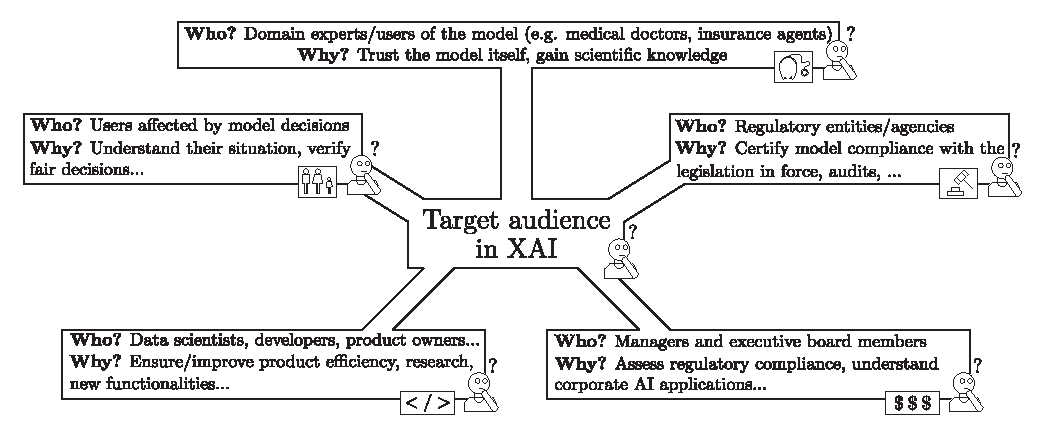
\includegraphics[trim={0.1cm 0.1cm 0.1cm
    0.1cm},clip,width=14cm]{pdfs/borrowed/xai_target_audience.pdf}
  \caption{Examples of various target audiences in XAI; figure taken from
    \citet{arrieta2020explainable}}
  \label{fig:xai_target_audience}
\end{figure}

\subsection{Terminology clarification}

\label{section:xai_terminology}

Based on their extensive literature review, \citet{arrieta2020explainable}
observe that many studies tend to misuse the terms interpretability and
explainability by using them interchangeably. To address this, they provide
clear conceptual differences between the terms. For example, \citet[Page 3,
Section 2.1]{arrieta2020explainable} state that \textit{``interpretability
  refers to a passive characteristic of a model referring to the level at which
  a given model makes sense for a human observer.''} In contrast, \citet[Page 3,
Section 2.1]{arrieta2020explainable} state that \textit{``explainability can be
  viewed as an active characteristic of a model, denoting any action or
  procedure taken by a model with the intent of clarifying or detailing its
  internal functions.''}

In summary, we gather that interpretability (or transparency as per Remark
\ref{rmk:equivalence}) refers to an inherent or passive feature of a model. On
the other hand, explainability refers to an active characteristic undertaken by
the model and its developers to explain the model's inner mechanisms. In
addition, explainability entails the presence of a target audience; which may
not necessarily be the case for interpretability or transparency.

\subsection{Post-hoc explainability techniques}

\label{section:xai_techniques}

Based on the aforementioned classification of \ac{ml} models into transparent and
black-box models, \citet{arrieta2020explainable} expound on explainability
techniques for each of these model types. Due to their transparent nature, the
study states that transparent \ac{ml} models are usually explainable in themselves to
most target audiences and therefore usually do not require any external
technique to extract explanations. The study does however highlight some target
audiences, such as non-expert users, who may require external explainability
techniques such as model output visualizations in order to explain the inner
workings of transparent \ac{ml} models.

For the case of black-box models, \citet{arrieta2020explainable} argue that
separate or external techniques must be utilized in order to reasonably explain
these models. Such explainability techniques are referred to in the study as
post-hoc explainability techniques; which is derived from the idea that
explanations for such models are usually extracted post-modeling. Notable
examples of post-hoc explainability techniques include local explanations,
feature relevance and explanations by simplification; for which we provide
adapted definitions below.

\begin{definition}[Local explanations; \citealt{arrieta2020explainable}; Page 11,
  Section 4.1]
  Local explanations operate by segmenting a model's solution space into
  subspaces and provide explanations for the less complex model subspaces.
\end{definition}

\begin{remark}
  Local explanations are commonly used in \ac{xai} research and function by using
  differentiating properties on model solution space subsets.
\end{remark}

\begin{remark}
  Two well-known examples of local explainability techniques are Local
  Interpretable Model-Agnostic Explanations \citep{lime} and G-REX
  \citep{konig2008g}.
\end{remark}

\begin{definition}[Feature relevance; \citealt{arrieta2020explainable}; Page 11,
  Section 4.1]
  Feature relevance explanation methods operate by computing an importance score
  for the model's input features over the model's outputs. These
  scores typically quantify how sensitive the model's output is to perturbations
  in the model's inputs or internal features.
\end{definition}

\begin{remark}
  Feature relevance methods can be considered as indirect methods of explaining
  a model.
\end{remark}

\begin{remark}
  Well-known feature relevance explainability techniques include the Shapley
  Additive Explanations \citep{lundberg2017unified} and the occlusion
  sensitivity method \citep{zeiler2014visualizing}.
\end{remark}

\begin{definition}[Explanations by simplification;
  \citealt{arrieta2020explainable}; Page 11, Section 4.1]
  \label{def:explain_simplify}
  Explanations by simplification refer to techniques where a simplified proxy
  model is built to approximate and explain a more complex model. The simplified
  proxy model usually has to fulfil the the joint criteria of reducing its
  complexity compared to its antecedent model while maximizing its resemblance
  to its antecedent and keeping a similar performance score.
\end{definition}

\begin{remark}
  In this thesis, we refer to the original black-box model as an
  \textit{antecedent} model and the simplified model as the \textit{proxy}
  model. Furthermore, we qualify that all proxy models must be designed to
  globally approximate their respective antecedent models.
\end{remark}

\begin{remark}
  \citet{bastani2017interpretability} and \citet{tan2018distill} are examples of
  studies that extract and distill simpler proxy models from complex antecedent
  models.
\end{remark}

Through our own survey of recent literature on explainability techniques used in
\ac{nlp}, we came across several interesting studies employing the local
explanations, feature relevance and explanations by simplification
explainability techniques to better explain black-box models; particularly deep
neural networks.
\citep{schwartz2018sopa,peng2018rational,suresh-etal-2019-distilling,wang2019state,jiang2020cold}.
We expound more on these in Sections \ref{section:fa} and \ref{section:sopa}
respectively.

\begin{figure}[t]
  \centering
  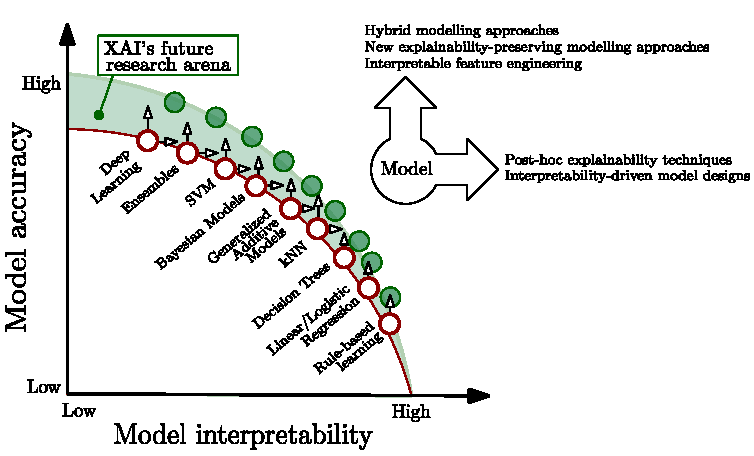
\includegraphics[width=14cm]{pdfs/borrowed/performance_transparency_tradeoff.pdf}
  \caption{Qualitative visualization of the performance-interpretability tradeoff;
    figure taken from \citet{arrieta2020explainable}}
  \label{fig:performance_interpretability_tradeoff}
\end{figure}

\subsection{Performance-interpretability tradeoff}

\label{section:performance_interpretability_tradeoff}

An interesting and insightful contribution of \citet{arrieta2020explainable} is
their conceptualization of the performance-interpretability tradeoff; which in
its essence states that the interpretability or transparency of models is
negatively correlated with performance on \ac{ml} tasks. \citet[Page 18, Section
5.1]{arrieta2020explainable} introduce the performance-interpretability tradeoff
with the caveat that \textit{``the matter of interpretability versus performance
  is one that repeats itself through time, but as any other big statement, has
  its surroundings filled with myths and misconceptions.''} To address some of
the aforementioned myths and misconceptions, \citet{arrieta2020explainable}
first disprove the generic statement that black-box models are
\textit{always} more performant by pointing to case studies which show that
transparent models can perform on-par or better than black-box models when the
function to be modeled is simple, data is well-structured and input
features are available with high quality.

With these exceptions clarified, \citet{arrieta2020explainable} then provide cases
which show that black-box models perform better than transparent models; which
ultimately gives rise to the performance-interpretability tradeoff as
reflected in Figure \ref{fig:performance_interpretability_tradeoff}. According to
them, this is usually the case when the function to be modeled is sufficiently
complex and where the input data has high diversity or variance; and possibly
contains significant noise.

\subsection{Explainability metrics}

\label{section:xai_metrics}

Towards the end of their study, \citet{arrieta2020explainable} note two major
limitations of the current state of \ac{xai} research. Firstly, they observe the lack
of a unified conceptualization of explainability and transparency between
various studies. To address this, they acknowledge that their study could
provide a good unified starting point for other \ac{xai} studies to branch out from.
Secondly, \citet{arrieta2020explainable} note the lack of a unified metric that
denotes how explainable any given model is. They explain why developing
such a metric has been a difficult process for many \ac{xai} studies; particularly
because such a metric would entail incorporating psychological, sociological and
cognitive elements to accommodate the goodness of fit of an explainability
technique to a certain target audience. Furthermore, incorporating such elements
might involve significant amounts of subjectivity in the desired metric.

To reduce some of the aforementioned subjectivity involved, \citet{MILLER20191}
and \citet{arrieta2020explainable} provide three guidelines of what could
constitute a good explanation based on human psychology, sociology and cognitive
sciences:

\begin{enumerate}
  \item Firstly, they observe that explanations are better when
  \textit{constrictive}; meaning an explanation is good if it not only explains
  why a model made decision X, but also why it made decision X over decision Y.

  \item Next, they suggest that good explanations should be able to communicate
  \textit{causal} links over probabilities; which could be a challenge for black-box
  models which generally compute aggregate probabilities without necessarily
  considering causal links.

  \item Finally, they recommend that explanations are better when
  \textit{selective}; meaning that a good explanation should be able to
  selectively provide the most important causal links instead of all possible
  causal links as these might be irrelevant or confusing to the target audience.
\end{enumerate}

\section{Straight-through estimator}

\label{section:ste}

Quantized neural networks refer to neural networks that contain
layers which transmit piecewise discrete signals and have been an object of
active research in regards to low-precision and low-resource computing. One of
the main challenges in training such quantized neural networks is
that their gradients tend to vanish almost everywhere because the derivatives of
such piecewise discrete activation functions typically default to zero
\citep{bengio2013estimating,courbariaux2016binarized,yin2019understanding}.

One significant workaround for this issue was proposed by
\citet{bengio2013estimating} through the introduction of the \ac{ste}. In the
vanilla version of the \ac{ste}, the \ac{ste} neuron emits a signal of 1 when its input is
strictly positive, and emits a zero signal in all other cases (Equation
\ref{eq:ste_forward}). The \ac{ste} then uses a simple identity function to estimate
the gradient during the backward pass (Equation \ref{eq:ste_backward}). The
vanilla \ac{ste} is visualized in Figure \ref{fig:ste}.

\begin{equation}
  \label{eq:ste_forward}
  \text{STE}(x)=
  \begin{cases}
    1 & x \in (0, +\infty) \\
    0 & x \in (-\infty, 0]
  \end{cases}
\end{equation}

\begin{equation}
  \label{eq:ste_backward}
  \text{STE}'(x)= x
\end{equation}

\begin{figure}[t]
  \centering
  \includegraphics[width=14cm]{pdfs/generated/ste_theoretical/main.pdf}
  \caption{Visualization of the vanilla STE's forward and backward passes}
  \label{fig:ste}
\end{figure}

Aside from the vanilla \ac{ste}, several other flavors of \ac{ste}s have been proposed by
studies such as \citet{courbariaux2016binarized} and
\citet{yin2019understanding}. In general, these studies have shown that
quantized neural networks perform competitively with their
non-quantized counterparts; while providing performance-related benefits related
to lower precision computing as well as enabling further research into threshold
driven neural activation functions.

\section{Finite-state automata}

\label{section:fa}

As mentioned in Section \ref{section:xai_techniques}, our survey of
explainability in \ac{nlp} yielded several studies employing a post-hoc
explainability techniques on deep neural networks. One common factor among
several of these studies was the simplification of black-box models to
\ac{fas}. As this will eventually become a key focus of this
thesis, we define key concepts related to the \ac{fas}; as well as extensions to \ac{fas}.

\subsection{Finite-state automaton}

Finite-state automata is a collective term for two sub-categories of models;
namely deterministic and nondeterministic finite-state automata. Here we provide
definitions and descriptions for these mutually exclusive model categories.

\begin{definition}[Deterministic finite-state automaton;
  \citealt{sipser1996introduction}]
  \label{def:fa}
  A deterministic finite-state automaton is a 5-tuple $\mathcal{M} = \langle
  \Sigma, \mathcal{Q}, \delta, q_0, F \rangle$, with:
  \begin{itemize}
    \itemsep0em
    \item[--] a finite input alphabet $\Sigma$;
    \item[--] a finite state set $\mathcal{Q}$;
    \item[--] a transition function $\delta: \mathcal{Q} \times \Sigma
    \rightarrow \mathcal{Q}$;
    \item[--] an initial state $q_0 \in \mathcal{Q}$;
    \item[--] and a set of final or accepting states $F \subseteq Q$.
  \end{itemize}
\end{definition}

\begin{definition}[Nondeterministic finite-state automaton;
  \citealt{sipser1996introduction}]
  \label{def:nfa}
  A nondeterministic finite-state automaton is a 5-tuple $\mathcal{M} = \langle
  \Sigma, \mathcal{Q}, \delta, q_0, F \rangle$, with:
  \begin{itemize}
    \itemsep0em
    \item[--] a finite input alphabet $\Sigma$;
    \item[--] a finite state set $\mathcal{Q}$;
    \item[--] a transition function $\delta: \mathcal{Q} \times \{\Sigma \cup
    \{\epsilon\}\} \rightarrow \mathcal{P}(\mathcal{Q})$;
    \item[--] an initial state $q_0 \in \mathcal{Q}$;
    \item[--] and a set of final or accepting states $F \subseteq Q$.
  \end{itemize}

  \begin{remark}
    $\epsilon \notin \Sigma$ refers to an empty-string transition
    and results in a change of state without consuming any input
    token. These transitions are unique to nondeterministic finite-state automata.
  \end{remark}

  \begin{remark}
    Self-loop transitions refer to special transitions which consume an input token
    while staying at the same state. These are allowed in both deterministic and
    nondeterministic finite-state automata.
  \end{remark}
  
  \begin{remark}
    $\mathcal{P}(\mathcal{Q})$ refers to the power set of $\mathcal{Q}$, or
    otherwise the collection of all subsets of $\mathcal{Q}$.
  \end{remark}
\end{definition}

\begin{definition}[Linear-chain finite-state automaton;
  \citealt{schwartz2018sopa}]
  \label{def:lfa}
  Any finite-state automaton is considered linear-chain if there exists only one
  set of consecutive transition states leading from the start to the accepting
  state. Linear-chain finite-state automata furthermore possess only one start
  and accepting state and only allow transitions to the same or next state which is
  closer to the accepting state.

  \begin{remark}
    \label{rmk:strict_linear_chain}
    A linear-chain finite-state automaton can be considered as \textit{strict}
    if it does not permit self-loop transitions and therefore only permits
    transitions to adjacent states which are strictly closer to the
    accepting state. An example of a strict linear-chain \ac{nfa} can be seen in
    Figure \ref{fig:regex_fa}.
  \end{remark}

  \begin{remark}
    The presence of the linear-chain terminology is effectively absent in
    theoretical computer science literature but is prevalent in practical
    research related to Hidden Markov Models and Conditional Random
    Fields such as in \citet{tsuruoka2009fast}. As a result, we are only
    able to provide a text-based definition here.
  \end{remark}
  
\end{definition}

A string $\bm{x}$ is said to be \textit{accepted} by any \ac{fa} $\mathcal{M}$ if the
current state after consuming string $\bm{x}$ is the accepting state. Similarly,
a string $\bm{x}$ is said to be \textit{rejected} by any \ac{fa} $\mathcal{M}$ if the
string $\bm{x}$ cannot be consumed or the current state after consuming $\bm{x}$
is a non-accepting state. The key difference between deterministic \ac{fas} and
non-deterministic \ac{fas} is present in
their transition functions; specifically that the former guarantees that each
state allows for a unique transition to another state given a non-empty input
string. Contrastingly, \ac{nfas} allow for arbitrary transitions without necessarily
consuming an input token.

\begin{figure}[t]
  \centering
  \includegraphics[width=14cm]{pdfs/generated/re_nfa_linear_chain/main.pdf}
  \caption{Regular expression \texttt{``how are (you|they) doing ?''} converted
    into a strict linear-chain NFA; double circles on state 5 indicate an
    accepting state}
  \label{fig:regex_fa}
\end{figure}

\subsection{Regular expressions}

Regular expressions and \ac{fas} have been shown to be equivalent in their
expressive power in that they both recognize regular languages
\citep{sipser1996introduction}. Historically, several algorithms have been
studied and optimized for converting \ac{fas} to regular expressions and vice-versa
\citep{mcnaughton1960regular,thompson1968programming}. Figure \ref{fig:regex_fa}
shows a simple example of converting the regular expression \texttt{``how are
  (you|they) doing ?''} into a strict linear-chain \ac{nfa}. The aforementioned
regular expression is written using the Perl-compatible regular expression
syntax with the \texttt{``|''} character indicating alternative possibilities.

\subsection{Weighted finite-state automaton}

\ac{wfas} are extensions of finite-state automata
which allow for the assignment of numerical weights to transitions given a
semiring to govern the algebra of the transitions. Compared to
the aforementioned \ac{fas} that only accept or reject strings, \ac{wfas} numerically
score strings which has made them useful for several applications in \ac{nlp} such as
tokenization and part-of-speech tagging \citep{maletti2017survey}. Here, we provide
extensive definitions of a semiring, \ac{wfa}, path score and string score.

\begin{definition}[Semiring; \citealt{kuich1986linear}]
  \label{def:semiring}
  A semiring is a set $\mathbb{K}$ along with two binary associative operations
  $\oplus$ (addition) and $\otimes$ (multiplication) and two identity elements:
  $\bar{0}$ for addition and $\bar{1}$ for multiplication. Semirings require
  that addition is commutative, multiplication distributes over addition, and
  that multiplication by $\bar{0}$ annihilates, i.e., $\bar{0} \otimes a = a
  \otimes \bar{0} = \bar{0}$.

\begin{remark}
  Semirings follow the following generic notation: $\langle \mathbb{K}, \oplus,
  \otimes, \bar{0}, \bar{1} \rangle$.
\end{remark}

\begin{remark}
  A simple and common semiring is the real or sum-product semiring: $\langle
  \mathbb{R}, +, \times, 0, 1 \rangle$. Two important semirings for this thesis
  are shown below.
\end{remark}

\begin{remark}
  \textbf{Max-sum} semiring: $\langle \mathbb{R} \cup \{-\infty\}, \text{max},
  +, -\infty, 0 \rangle$
\end{remark}

\begin{remark}
  \textbf{Max-product} semiring: $\langle \mathbb{R}_{>0} \cup \{-\infty\},
  \text{max}, \times, -\infty, 1 \rangle$
\end{remark}

\end{definition}

\begin{definition}[Weighted finite-state automaton; \citealt{peng2018rational}]
  \label{def:wfa}
  A weighted finite-state automaton over a semiring $\mathbb{K}$ is a 5-tuple
  $\mathcal{A} = \langle \Sigma, \mathcal{Q}, \bm{\Gamma}, \bm{\lambda}, \bm{\rho} \rangle$,
  with:

  \begin{itemize}
    \itemsep0em
    \item[--] a finite input alphabet $\Sigma$;
    \item[--] a finite state set $\mathcal{Q}$;
    \item[--] transition matrix $\bm{\Gamma}: \mathcal{Q} \times \mathcal{Q} \times
    (\Sigma \cup \{\epsilon\}) \rightarrow \mathbb{K}$;
    \item[--] initial vector $\bm{\lambda}: \mathcal{Q} \rightarrow \mathbb{K}$;
    \item[--] and final vector $\bm{\rho}: \mathcal{Q} \rightarrow \mathbb{K}$.
  \end{itemize}

  \begin{remark}
    $\Sigma^{*}$ refers to the (possibly infinite) set of all strings over the
    alphabet $\Sigma$, where * represents the Kleene star operator.
  \end{remark}

  \begin{remark}
    As with finite-state automata, it is also possible to construct (strict)
    linear-chain weighted finite-state automata. Similarly, it is possible to
    extract a \ac{fa} from a \ac{wfa} given a particular set of valid transitions.
  \end{remark}
 
\end{definition}

\begin{definition}[Path score; \citealt{peng2018rational}]

  Let $\bm{\pi} = \langle \pi_1, \pi_2, \dots, \pi_n \rangle$ be a sequence of
  adjacent transitions in $\mathcal{A}$, with each $\pi_i = \langle q_i,
  q_{i+1}, z_i \rangle \in \mathcal{Q} \times \mathcal{Q} \times (\Sigma \cup
  \{\epsilon\})$. The path $\bm{\pi}$ derives the $\epsilon$-free string
  $\bm{x} = \langle x_1, x_2, \dots, x_m \rangle \in \Sigma^{*}$; which is a
  substring of the $\epsilon$-containing string $\bm{z} = \langle z_1, z_2,
  \dots, z_n \rangle \in (\Sigma \cup \{\epsilon\})^{*}$. $\bm{\pi}$'s score in
  $\mathcal{A}$ is given by:
  
\end{definition}

\begin{equation}
  \mathcal{A}[\bm{\pi}] = \bm{\lambda}(q_1) \otimes \Bigg( \bigotimes_{i=1}^n \bm{\Gamma}(\pi_i) \Bigg) \otimes \bm{\rho}(q_{n+1})
\end{equation}

\begin{definition}[String score; \citealt{peng2018rational}]
  \label{def:string_score}
  Let $\Pi(\bm{x})$ denote the set of all paths in $\mathcal{A}$ that derive
  $\bm{x}$. Then the string score assigned by $\mathcal{A}$ to string $\bm{x}$
  is given by:
  
\end{definition}

\begin{equation}
  \mathcal{A}[\![\bm{x}]\!] = \bigoplus_{\bm{\pi} \in \Pi(\bm{x})} \mathcal{A}[\bm{\pi}]
\end{equation}

\begin{remark}
  Since $\mathbb{K}$ is a semiring, $\mathcal{A}[\![\bm{x}]\!]$ can be
  efficiently computed using the Forward algorithm \citep{baum1966statistical}.
  Its dynamic program is summarized below without $\epsilon$-transitions for
  simplicity. $\Omega_i(q)$ gives the aggregate score of all paths that derive
  the substring $\langle x_1, x_2, \dots, x_i \rangle$ and end in state $q$:
 
  \begin{subequations}
    \begin{align}
      \Omega_0(q) &= \bm{\lambda}(q) \\
      \Omega_{i+1}(q) &= \bigoplus_{q' \in \mathcal{Q}} \Omega_i(q') \otimes \bm{\Gamma}(q',q,x_i)  \\
      \mathcal{A}[\![\bm{x}]\!] &= \bigoplus_{q \in \mathcal{Q}} \Omega_n(q) \otimes \bm{\rho}(q)
    \end{align}
  \end{subequations}

\end{remark}

\begin{remark}
  \label{rmk:old_runtime}
  The Forward algorithm can be generalized to any semiring
  \citep{eisner2002parameter} and has a runtime of $O(|Q|^3 + |Q|^2|\bm{x}|)$
  \citep{schwartz2018sopa}; notably with a linear runtime with respect to the
  length in tokens of the input string $\bm{x}$.
\end{remark}

\begin{remark}
  A special case of Forward is the Viterbi algorithm, where the addition
  $\oplus$ operation is constrained to the maximum operator
  \citep{viterbi1967error}. Viterbi therefore returns the highest scoring path
  $\bm{\pi}$ that derives the input string $\bm{x}$.
\end{remark}

\section{SoPa}

\label{section:sopa}

As mentioned previously in Chapter \ref{chapter:introduction}, a key focus of
this thesis is in improving the \textbf{So}ft \textbf{Pa}tterns (SoPa) model
presented in \citet{schwartz2018sopa}. In this section, we describe important
aspects of the SoPa model which ultimately become relevant for our
methodologies. \citet{schwartz2018sopa} introduce SoPa as a novel and
lightweight hybridized \ac{rnn}, \ac{cnn} and \ac{wfa}-based neural architecture. SoPa
resembles a \ac{rnn} because it processes text sequentially and can encode strings of
arbitrary lengths. Similarly, the architecture contains a variable number of
constrained linear-chain \ac{wfas} with variable numbers of states or window sizes;
which resembles both one-layer \ac{cnn}s and an ensemble of linear-chain \ac{wfas}. The
combination of the aforementioned features ultimately allows SoPa to learn soft
versions of traditionally hard surface patterns.

In their study, \citet{schwartz2018sopa} test the SoPa architecture on three
separate sentiment classification tasks and compare the results with four
baselines which include a bidirectional \ac{lstm} and a \ac{cnn}. With their results, they
show that SoPa performed on par or better than all baselines on all tasks.
Additionally, they show that SoPa outperformed all baselines significantly in
low-data settings. Finally, the authors present workflows to explain the SoPa
model using both the local explanations and feature relevance explainability
techniques.

\begin{figure}[t]
  \centering
  \includegraphics[width=14cm]{pdfs/generated/generic_nfa_linear_chain/main.pdf}
  \caption{Visualization of a (non-strict) linear-chain NFA with
    self-loop (blue), $\epsilon$ (red) and main-path (black) transitions; figure
    adapted from \citet{schwartz2018sopa}}
  \label{fig:fa}
\end{figure}

\subsection{Linear-chain WFAs}

\label{section:sopa_lc_wfa}

In regards to the \ac{wfas} used in SoPa, \citet{schwartz2018sopa} utilize
linear-chain \ac{wfas} where each linear-chain \ac{wfa} is alloted a sequence of
$|\mathcal{Q}|$ states. Each state $i$ in the linear-chain \ac{wfa} has three
possible outgoing transitions; namely a \textbf{self-loop transition} which
consumes a token but stays in the same state $i$, an
\textbf{$\bm{\epsilon}$-transition} which does not consume a token but transitions to
state $i+1$ and a \textbf{main-path transition} which consumes a specific token
and transitions to state $i+1$. Furthermore, \citet{schwartz2018sopa} utilize
only the max-sum and max-product semirings in their linear-chain \ac{wfas}. Figure
\ref{fig:fa} shows a sample \ac{nfa} extracted from the aforementioned linear-chain
\ac{wfa} with all three aforementioned transitions, which could accept
strings such as \texttt{"what a great book !"} and \texttt{"what a great
  entertaining book !"}.

To more concretely express these transitions, \citet{schwartz2018sopa} provide
the following formulation of the transition matrix $\bm{\Gamma}$ under the
linear-chain structure. Here, $\bm{\Gamma}(x)$ represents a $|Q|\times|Q|$ matrix
containing transition scores when consuming an input token $x$. $[\bm{\Gamma}(x)]_{i,j}$
corresponds to the cell value in $\bm{\Gamma}(x)$ for row $i$ and column
$j$ and represents the transition score when consuming token $x$ and
transitioning from state $i$ to $j$.

\begin{equation}
  \label{eq:sopa_transition_matrix_main}
  [\bm{\Gamma}(x)]_{i,j} =
  \begin{cases}
    \bm{u}_i \cdot \bm{v}_x + a_i  & \text{if } j = i \text{ (self-loop transition),} \\
    \bm{w}_i \cdot \bm{v}_x + b_i  & \text{if } j = i + 1 \text{ (main-path transition),} \\
    \bar{0} & \text{otherwise.}
  \end{cases}
\end{equation}

Here, $\bm{u}_i$ and $\bm{w}_i$ are learnable vectors and $a_i$ and $b_i$ are
learnable scalar biases parameterizing transitions out of state $i$. $\bm{v}_x$
represents the word embedding for token $x$ and $\bar{0}$ represents the zero
value in the semiring used as per Definition \ref{def:semiring}. Similarly,
$\epsilon$-transitions are parameterized with the following representation in
$\bm{\Gamma}$:

\begin{equation}
  \label{eq:sopa_transition_matrix_epsilon}
  [\bm{\Gamma}(\epsilon)]_{i,j} =
  \begin{cases}
    c_i  & \text{if } j = i + 1 \text{ ($\epsilon$-transition)} \\
    \bar{0} & \text{otherwise.}
  \end{cases}
\end{equation}

Here, $c_i$ represents a learnable scalar bias for $\epsilon$-transitions out of
state $i$. Next, \citet{schwartz2018sopa} fix the initial vector $\bm{\lambda} =
[\bar{1}, \bar{0}, \ldots, \bar{0}]$ and the final vector $\bm{\rho} = [\bar{0},
\bar{0}, \ldots, \bar{1}]$, where $\bar{1}$ and $\bar{0}$ represent the one and
zero values specified in the semiring as per Definition \ref{def:semiring}.
Ultimately, these are formalisms to imply that there only exists one start and
one accepting state and these are present at both extremes of the linear-chain
\ac{wfa}; which is ultimately consistent with the linear-chain definition as per Definition
\ref{def:lfa}.

The aforementioned constraints in the linear-chain \ac{wfa} structure result in the
transition matrix $\bm{\Gamma}$ being reduced to a sparse diagonal matrix.
Correspondingly, the runtime of the Forward algorithm under the linear-chain
\ac{wfas} gets reduced to $O(|Q||\bm{x}|)$ compared to the original runtime in
Remark \ref{rmk:old_runtime}. Finally, it is worth noting that \citet[Page 3,
Section 3.1]{schwartz2018sopa} refer to the linear-chain \ac{wfas} simply as
\textit{``patterns''}. For brevity and consistency, we refer to linear-chain
\ac{wfas} as patterns interchangeably.

\subsection{Document score}

\label{section:sopa_doc_score}

Since SoPa was intended to compute scores for entire documents and not just
short strings, \citet[Page 3, Section 3.2]{schwartz2018sopa} propose computing
the string score, as per Definition \ref{def:string_score}, over all consecutive
substrings in the document which ultimately returns a document score
$s_{\text{doc}}(\bm{y})$ for an arbitrary document $\bm{y}$. The document score
$s_{\text{doc}}(\bm{y})$ for a \ac{wfa} would represent an aggregated score over all
consecutive substrings and would therefore also depend on the semiring used in
the \ac{wfas}. In the case of max-based semirings using the Viterbi algorithm, the
document score $s_{\text{doc}}(\bm{y})$ would reflect the highest path score
corresponding to a substring in document $\bm{y}$.

\subsection{Computational graph}

\label{section:sopa_cg}

To explain the overall computational graph of the SoPa model, we refer to the
visualization shown in Figure \ref{fig:sopa} with two \ac{wfas} highlighted in
blue and red. The \ac{wfas} compute the aforementioned document scores as they
traverse the document. Given max-based semirings, the max-pooled scores
accumulate in an output layer as shown on the top of Figure \ref{fig:sopa}.
After traversing the full document, the max-pooled scores are passed through a
\ac{mlp} which conducts the final classification to an output label. It is worth
noting that without $\epsilon$-transitions and self-loops, a linear-chain
\ac{wfa} with $|\mathcal{Q}|$ states should always consume $\mathcal{|Q|}-1$
tokens. However, by allowing the aforementioned special transitions; it is
possible for strings of variable lengths to be consumed since an
$\epsilon$-transition can transition to the next state without consuming tokens
while a self-loop can consume tokens without transitioning to the next state.
This is indeed the case for Pattern 2 in Figure \ref{fig:sopa}, when a self-loop
is encountered in the transition from the token \textit{``and''} to the token
\textit{``most''}.

\begin{figure}[t]
  \centering
  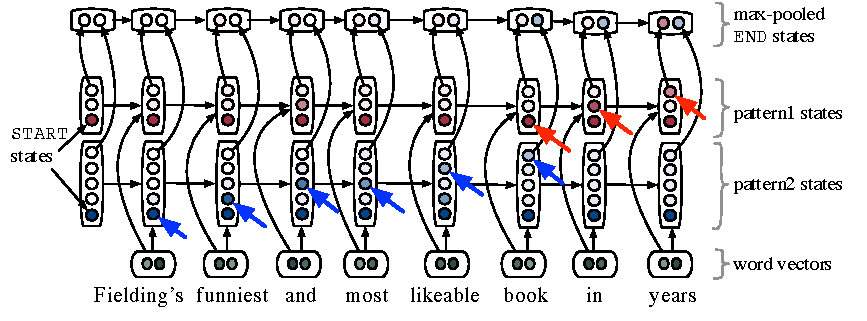
\includegraphics[width=14cm]{pdfs/borrowed/sopa_computational_graph.pdf}
  \caption{Visualization of the SoPa model framework with two constituent
    WFAs highlighted in blue and red; figure taken from
    \citet{schwartz2018sopa}}
  \label{fig:sopa}
\end{figure}

\subsection{Patterns hyperparameter $P$}

Training the SoPa model requires both commonly used and special hyperparameters.
Commonly used hyperparameters include the learning rate, neuron dropout and word
dropout probabilities. A special hyperparameter unique to the SoPa model is the
patterns hyperparameter $P$ which contains information on the number of
linear-chain \ac{wfas} and the number of states allotted to each of them. The
hyperparameter $P$ is encoded as a string with the following syntax:
\texttt{Length$_{1}$-Count$_{1}$\_$\dots$\_Length$_{k}$-Count$_{k}$}. An example
of this hyperparameter $P$ is \texttt{5-15\_4-10\_3-5}, which would signify 15
patterns with 5 states each, 10 patterns with 4 states each and 5 patterns with
3 states each.

\subsection{Transparency}

\label{section:sopa_transparency}

Since we expounded on \ac{xai} in Section \ref{section:xai} and made a case for
viewing \ac{ml} models from the lens of \ac{xai}, it would only make sense to extend the
same standards to the SoPa model. Based on the arguments made by
\citet{arrieta2020explainable}, we can classify the SoPa model as a black-box
model since it closely resembles \ac{rnn}s and \ac{cnn}s; and a strong case has already
been made in their study regarding the black-box natures of both \ac{rnn}s and \ac{cnn}s.
Naturally, this would imply that post-hoc explainability techniques are required to
explain the SoPa model.

\subsection{Explainability}

\label{section:sopa_post_hoc}

In their study, \citet[Page 7, Section 7]{schwartz2018sopa} describe two simple
post-hoc explainability techniques for the SoPa model. One method involves the
usage of back-pointers during the Viterbi computation to determine the patterns
and substrings in a document which contributed the highest pattern scores.
Another method involves zeroing out the corresponding patterns scores via the
occlusion sensitivity method to determine which pattern had the greatest impact
on each classification decision.

Using the post-hoc explainability taxonomies described in Section
\ref{section:xai_techniques}, we can correspondingly classify the explainability
techniques presented in \citet{schwartz2018sopa} using terminology consistent with
\ac{xai} research. The first explainability technique uses individual text samples to
determine the highest scoring substrings in documents; as well as the patterns
or \ac{wfas} corresponding to them. Since this analysis is conducted at an individual
document level and is never synthesized to a more global context, we would
classify this under the local explanations explainability technique. The next
technique involves an occlusion or sensitivity analysis over all patterns and
documents to determine which pattern had the greatest impact for each class.
Since this involves systematic perturbation to determine the importance of
pattern features, we would classify this technique as a feature relevance
explainability technique. While the target audience(s) of these
explainability techniques is not explicitly mentioned in their study, we infer that
the target audience for these techniques is likely to be end-users since the
outputs of these post-hoc explainability techniques are generally easy to understand.

In order to objectively probe the quality of the post-hoc explainability
techniques proposed by \citet{schwartz2018sopa}, we utilize the three guidelines
provided in Section \ref{section:xai_metrics}; namely that a good explanation
should be constrictive, causal and selective. For the constrictive quality, it
is likely that the explainability techniques do not meet this criterion since they
only highlight individual features that were important for SoPa, and do not
necessarily go into detail regarding why these features superseded adjacent
features. Next, the explainability techniques likely do not fulfill the criterion
of providing causal links; since they generally provide explanations by
aggregating probabilistic quantities inside SoPa. Finally and in
contrast, the explainability techniques likely pass the criterion of being
selective since they only provide the most important features for an
explanation.

%%% Local Variables: 
%%% mode: latex
%%% TeX-master: "main"
%%% End: 